\section{Process View}
De process view van het 4 + 1 model dient om het run-time gedrag van het systeem in beeld te brengen \parencite{4p1Model}.
In deze sectie wordt er gekeken hoe het ophalen van de data vanuit de backend werkt.
Verder wordt er ook gekeken hoe de data gerenderd wordt in de frontend.

\subsection{Backend}
Om het proces van het ophalen van de data in beeld te krijgen is er gebruik gemaakt van een sequencediagram.
In figuur \ref{fig:SequenceDiagramItemValueWithChildren} (vergrote afbeelding is te zien in \ref{appendix:SequenceDiagramItemValueWithChildren}) is te zien dat er 4 lagen zijn. 
Dit zijn de controller, datahandler, handler en repository.
De logica om te bepalen of het een succesvolle request was zit in de datahandler.
De verschillende handlers handelen de buisness logica af.
En als laatste is er de repository die de data uit de database haalt.

\whitespace
\begin{graphic}
    \captionsetup{type=figure}
    \caption{Sequencediagram ItemValue}
    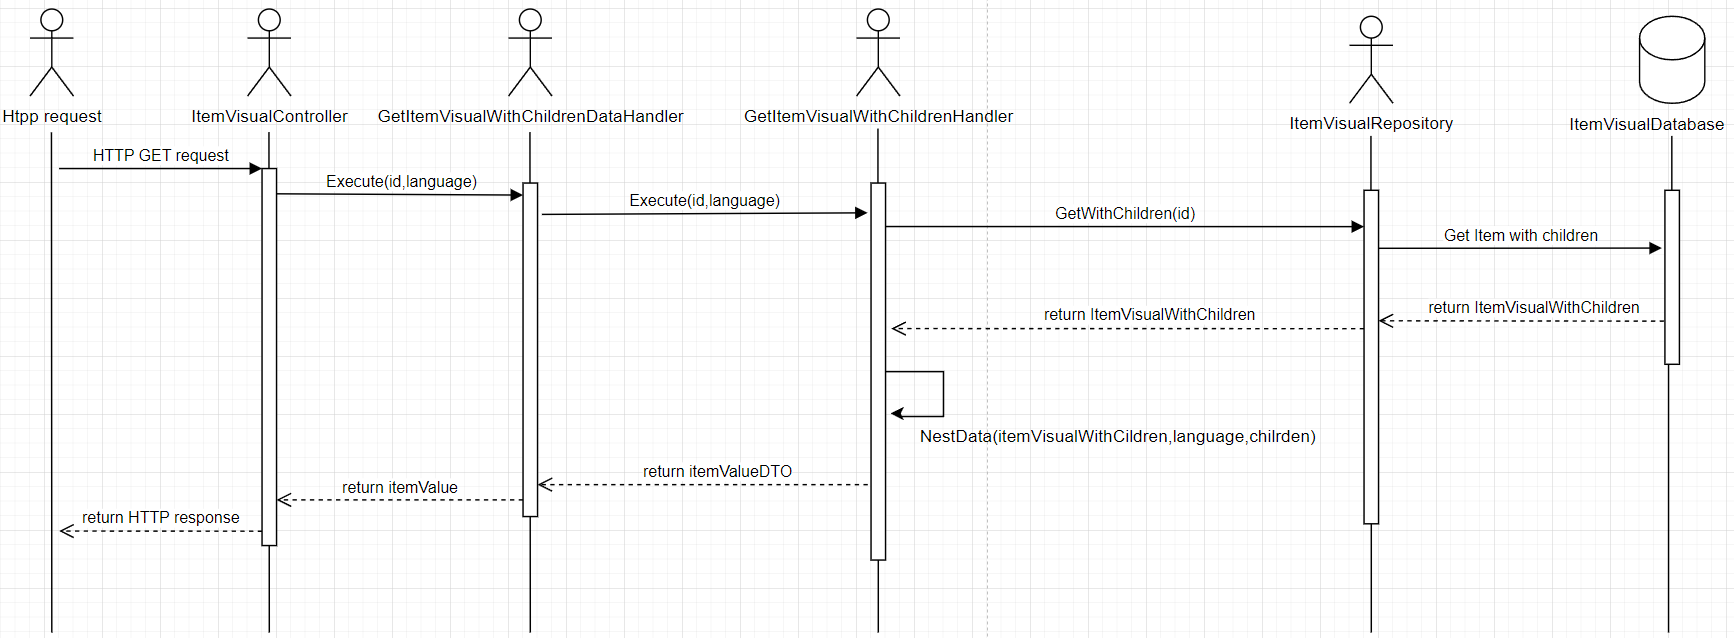
\includegraphics[scale=0.28]{SequenceDiagramItemValueWithChildren.png}
    \label{fig:SequenceDiagramItemValueWithChildren}
\end{graphic}

\newpage
\subsection{Frontend}
Om de geneste structuur van het datamodel te renderen wordt er gebruikgemaakt van 2 verschillende component types.
Deze component types worden appart toegelicht om een beter beeld te schetsen.

\whitespace[2]
\textbf{Type 1: Implementatie componenten}

\whitespace
Het eerste type componenten is het component dat daadwerkelijk de data rendered.
Deze componenten pakken de \textit{fields} van het \textit{item} en renderen dit op de frontend.
Als voorbeeld is er een stukje van de Snakeware site gepakt om dit beter toe te lichten (zie figuur \ref{fig:SingleComponent})
In dit voorbeeld wordt het titel field  gebruikt om de titel van het component te renderen.
En hetzelfde wordt ook gedaan voor het nummer en de body van het component.

\begin{graphic}
    \captionsetup{type=figure}
    \caption{Visualisatie implementatie component}
    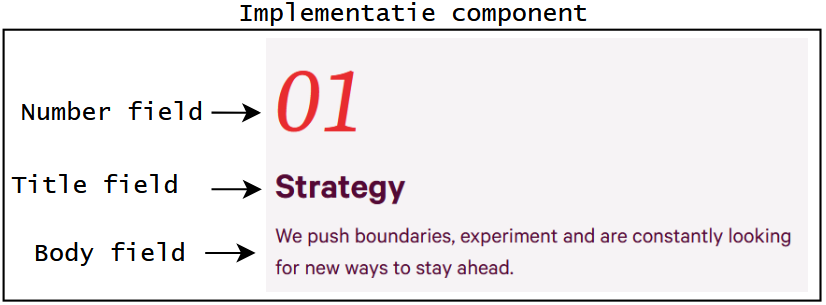
\includegraphics[scale=0.4]{ExampleDiffrentFrontendTypes.png}
    \label{fig:SingleComponent}
\end{graphic}

\whitespace[2]
\textbf{Type 2: Containers}

\whitespace
Omdat Implementatie componenten in elkaar genest kunnen zitten wordt er ook gebruik gemaakt van containers.
Containers zijn generieke componenten die een of meerdere implementatie componenten kan renderen.
Verder kunnen containers ook meerdere containers renderen.
Door dit te doen kunnen complexe structuren gerenderd.
Om hier een beter beeld bij te schetsen is het vorige voorbeeld (zie figuur \ref{fig:SingleComponent}) uitgebreid.
De uitgebreide versie is te zien in figuur \ref{fig:MultipleComponents}.

\whitespace
\begin{graphic}
    \captionsetup{type=figure}
    \caption{Visualisatie containers}
    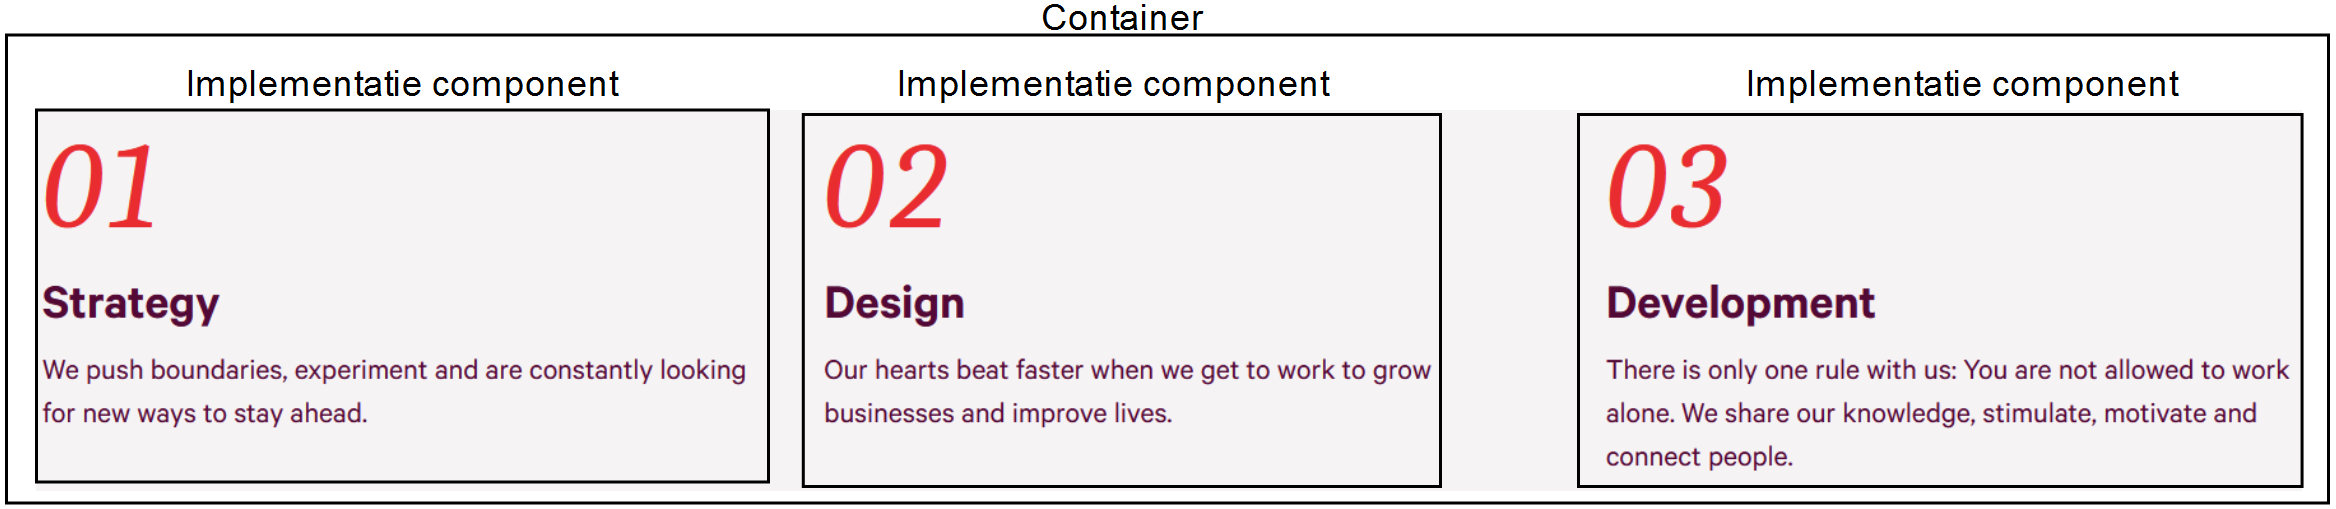
\includegraphics[scale=0.27]{ExampleContainerFrontend.png}
    \label{fig:MultipleComponents}
\end{graphic}
% Om de data te renderen wordt er gebruikgemaakt van 2 verschillende entiteiten types.
% Het eerste type zijn de voorgedefinieerde componenten in de frontend applicatie.
% Een voorbeeld hiervan zou kunnen zijn een artikel component.
% In figuur \ref{fig:VisualisationItems} is een artikel component te zien. 
% Deze componenten bevat de data van de verschillende items die gebruikt worden.
% Type 1 is een voor gedefinieerd component, hierbij kun je denken aan een artikel, card, afbeelding etc.
% Het andere type is een generiek component dat het type 1 componenten \textit{encapsulate}.
% Deze componenten worden containers genoemd omdat ze verschillende items encapsuleren.
% Verder kunnen containers ook meerdere containers encapsuleren.

\newpage
In figuur \ref{fig:FlowchartFrontend} wordt er getoond hoe de frontend met deze container structuur om gaat.
Na het ophalen van de data van de api wordt er meestal de root container gerendered.
Eerst wordt er gekeken of het huidige object 1 of meer items heeft.
Daarna wordt er gecontroleerd of het item een valide implementatie component heeft.
Als het item een container is dan wordt deze recursief gerenderd.
Dit wordt door gedaan tot dat alle items gerenderd zijn.

\whitespace
\begin{graphic}
    \captionsetup{type=figure}
    \caption{flowchart diagram frontend}
    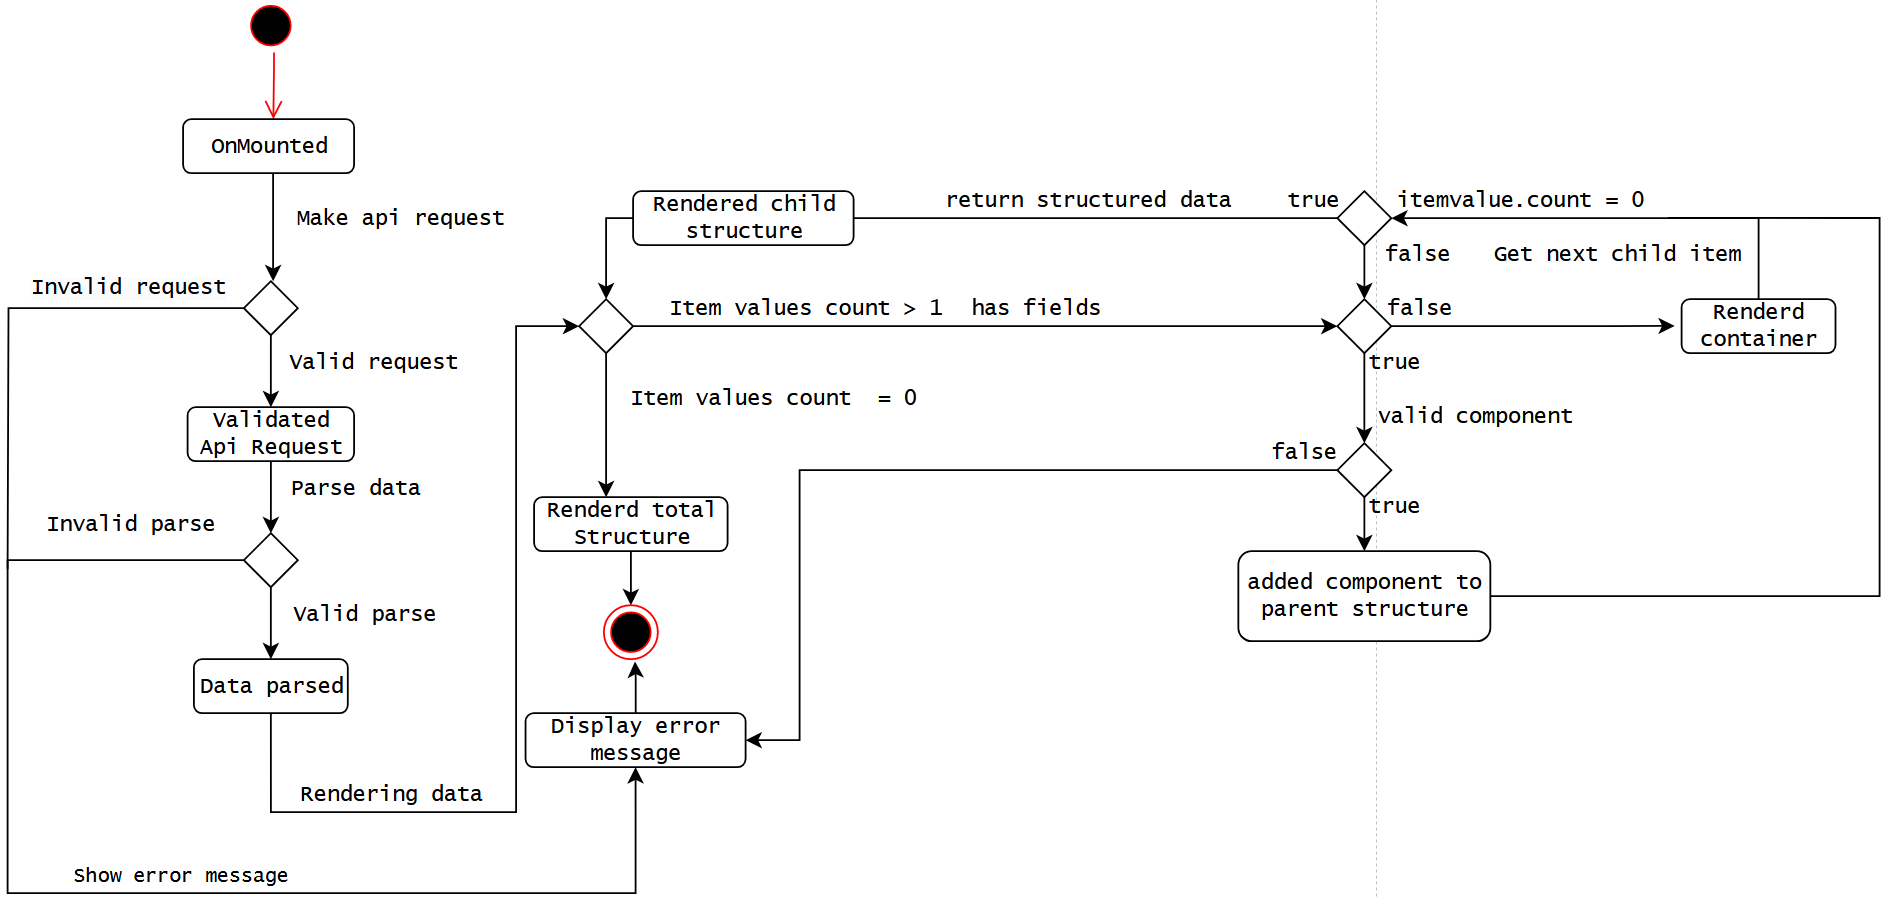
\includegraphics[scale=0.34]{FlowchartFrontend.png}
    \label{fig:FlowchartFrontend}
\end{graphic}
